\documentclass[border=12pt]{standalone}
\usepackage{tikz}
\usetikzlibrary{shapes.geometric, arrows.meta, positioning, calc, fit, backgrounds}
\usepackage{fontspec}
\setmainfont{DejaVu Sans}

\begin{document}
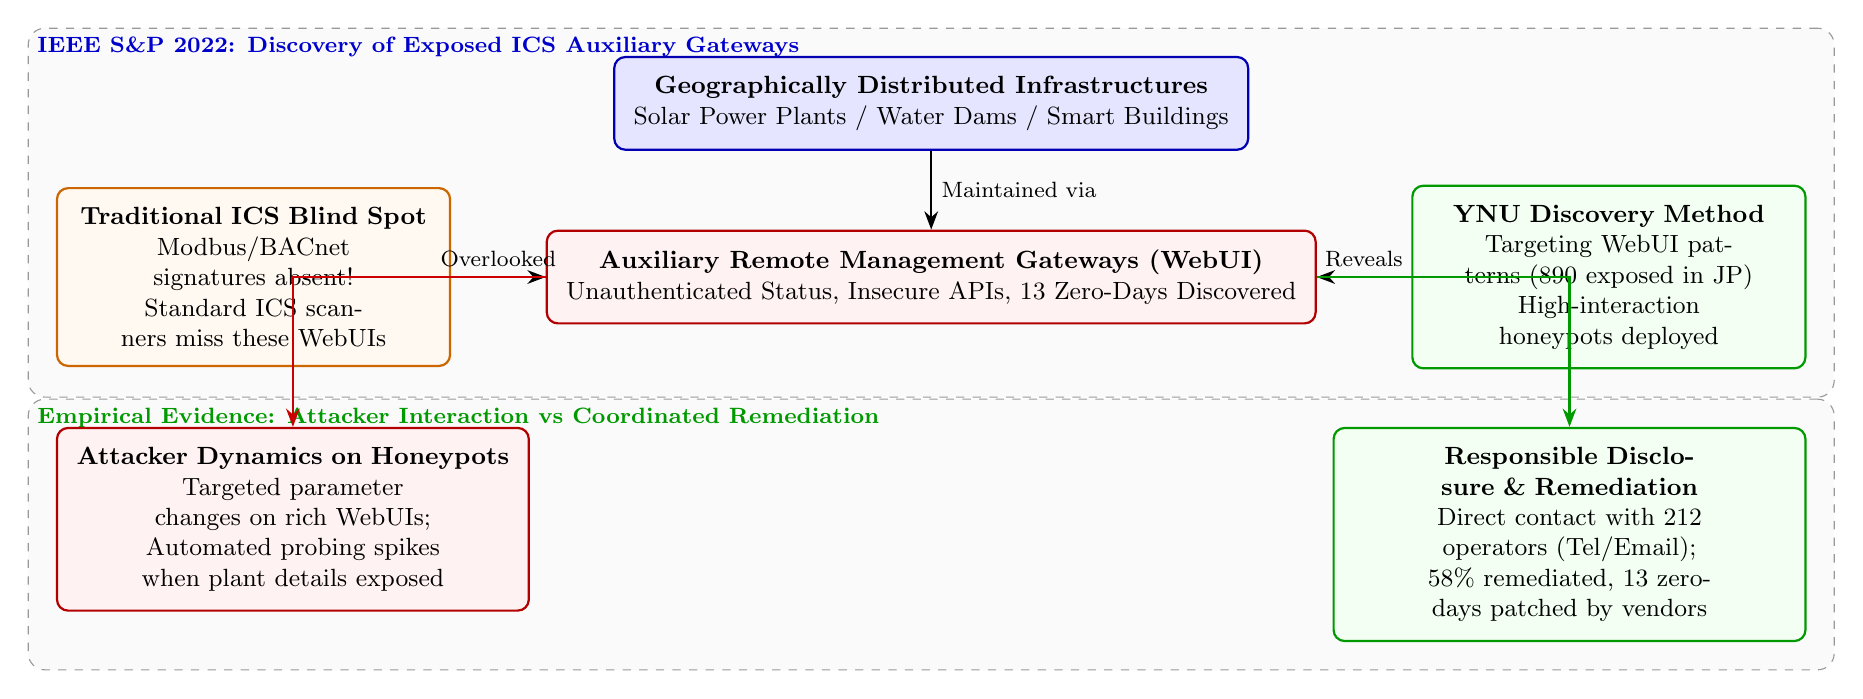
\begin{tikzpicture}[
    font=\small,
    >=Stealth,
    node distance=1.2cm,
    block/.style={rectangle, draw=blue!70!black, fill=blue!5, rounded corners=4pt, thick, align=center, inner sep=7pt},
    alertblock/.style={rectangle, draw=red!70!black, fill=red!5, rounded corners=4pt, thick, align=center, inner sep=7pt},
    greenblock/.style={rectangle, draw=green!60!black, fill=green!5, rounded corners=4pt, thick, align=center, inner sep=7pt},
    amberblock/.style={rectangle, draw=orange!80!black, fill=orange!5, rounded corners=4pt, thick, align=center, inner sep=7pt},
    groupbox/.style={draw=black!40, dashed, rounded corners=6pt, fill=black!2, inner sep=10pt}
]

    % Top Group: Critical Industrial Sites
    \node[block, fill=blue!10] (sites) {\textbf{Geographically Distributed Infrastructures}\\Solar Power Plants / Water Dams / Smart Buildings};

    % Insecure Gateways
    \node[alertblock, below=1.0cm of sites] (gateways) {\textbf{Auxiliary Remote Management Gateways (WebUI)}\\Unauthenticated Status, Insecure APIs, 13 Zero-Days Discovered};
    \draw[->, thick] (sites) -- node[right, font=\footnotesize] {Maintained via} (gateways);

    % Blind Spot & Discovery
    \node[amberblock, left=1.2cm of gateways, text width=4.5cm] (blindspot) {\textbf{Traditional ICS Blind Spot}\\Modbus/BACnet signatures absent!\\Standard ICS scanners miss these WebUIs};
    \draw[->, thick, dashed] (blindspot) -- node[above, font=\footnotesize] {Overlooked} (gateways);

    \node[greenblock, right=1.2cm of gateways, text width=4.5cm] (discovery) {\textbf{YNU Discovery Method}\\Targeting WebUI patterns (890 exposed in JP)\\High-interaction honeypots deployed};
    \draw[->, thick] (discovery) -- node[above, font=\footnotesize] {Reveals} (gateways);

    % Bottom Group: Attacker dynamics vs Responsible Remediation
    \node[alertblock, below left=1.3cm and 0.2cm of gateways, text width=5.5cm] (attackers) {\textbf{Attacker Dynamics on Honeypots}\\Targeted parameter changes on rich WebUIs;\\Automated probing spikes when plant details exposed};

    \node[greenblock, below right=1.3cm and 0.2cm of gateways, text width=5.5cm] (remediation) {\textbf{Responsible Disclosure \& Remediation}\\Direct contact with 212 operators (Tel/Email);\\58\% remediated, 13 zero-days patched by vendors};

    \draw[->, thick, red!80!black] (gateways) -| (attackers);
    \draw[->, thick, green!60!black] (gateways) -| (remediation);

    % Group backgrounds
    \begin{scope}[on background layer]
        \node[groupbox, fit=(sites) (gateways) (blindspot) (discovery), label={[anchor=north west, font=\footnotesize\bfseries, blue!80!black]north west:IEEE S\&P 2022: Discovery of Exposed ICS Auxiliary Gateways}] {};
        \node[groupbox, fit=(attackers) (remediation), label={[anchor=north west, font=\footnotesize\bfseries, green!60!black]north west:Empirical Evidence: Attacker Interaction vs Coordinated Remediation}] {};
    \end{scope}

\end{tikzpicture}
\end{document}
